%%%%% Document Setup %%%%%%%%

\documentclass[12pt, onecolumn]{revtex4}    % Font size (12pt) and column number (one or two).

\usepackage[a4paper, left=2.5cm, right=2.5cm, top=2.5cm, bottom=2.5cm]{geometry}  % Defines paper size and margin length

\renewcommand{\baselinestretch}{1}     % Defines the line spacing

\usepackage[caption=false]{subfig}

\usepackage{graphics,graphicx,epsfig,ulem}	% Makes sure all graphics works
\usepackage{amsmath} 						% Adds mathematical features for equations

\usepackage{etoolbox}                       % Customise date to preferred format
\makeatletter
\patchcmd{\frontmatter@RRAP@format}{(}{}{}{}
\patchcmd{\frontmatter@RRAP@format}{)}{}{}{}
\renewcommand\Dated@name{}
\makeatother

\usepackage{fancyhdr}

\pagestyle{fancy}                           % Insert header
\renewcommand{\headrulewidth}{0pt}
\lhead{\small }                        
\rhead{\small }                

\def\thesection{\arabic{section}}
\def\thesubsection{\alph{subsection}}

\def\bibsection{\section*{References}}        % Position reference section correctly
\setcitestyle{authoryear,round}
\setlength\bibhang{0.2in}
\usepackage[colorlinks]{hyperref}
\hypersetup{
    colorlinks=true,
    linkcolor=black,
    citecolor=black,    
    urlcolor=black,
}

\usepackage{tabularx}

%%%%% Document %%%%%
\begin{document}                     

\title{Prediction limitations with the spring predictability barrier in the Zebiak-Cane model for El Ni\~{n}o Southern Oscillations} 
%\date{Submitted: \today{}} \author{Jacky Cao}

\maketitle
\thispagestyle{plain} % produces page number for front 

\section{Introduction}
\noindent
% Introducing ENSOs and what EN and SO are individually and then setting the problem from the offset 
The El Ni\~{n}o Southern Oscillations (ENSOs) are a composite weather phenomena which originate and occur every few years in the Pacific Ocean. El Ni\~{n}o is an oceanic warming event which disrupts the normal Pacific circulation at irregular intervals of 2--7 years, whilst the Southern Oscillations are an inter-annual flip of the tropical sea level pressure between the western and eastern Pacific leading to the weakening and strengthening of the easterly oceanic trade winds \citep{wang2017nino}. The coupling of these two phenomena was first theorised by \cite{doi:10.1175/1520-04931969097} who recognised that they are two different aspects of the same phenomena. \\
% words: 97

% How Bjerknes, Zebiak and Cane set the stage for ENSO research 
Bjerknes hypothesised that a positive ocean-atmosphere feedback system would result in an El Ni\~{n}o event. An initial positive sea surface temperature (SST) anomaly in the eastern Pacific would reduce the east--west SST gradient which leads to the strengthening of the Walker circulation and the production of weaker trade winds across the equatorial Pacific. In a complete ENSO theory this positive system would be counterbalanced by a negative loop which returns the Pacific to its ``normal'' (pre-ENSO) state. \\
% words: 77

Whilst Bjerknes' theory failed to provide a negative feedback mechanism, \cite{Zebiak:1987aa} presented a model which would fill that void. In their work, they outlined an alternative atmosphere-ocean coupling mechanism. The atmospheric component was a linear Gill-type model \citep{Gill:1980aa} which describes the atmosphere's response to SST anomalies, and the ocean was represented by a low-gravity system which could be forced by atmospheric wind stress. \\
% words: 63

With their model, Zebiak and Cane were able to replicate features observed during ENSO events such as equatorial westerly wind anomalies in the central Pacific, large SST anomalies in the eastern Pacific, and were able to predict the onset of the 1986--1987 and 1991--1992 ENSO events. Despite this success, they recognised their limited ability in simulating a real system, thorough comparisons with observational data would reveal discrepancies in their atmospheric and oceanic simulations, and further simulations of the 1990s using the Zebiak-Cane (ZC) model would fail to predict the short warm episodes of 1993 and 1994. This culminated with the suggestion that more sophisticated models would be required to better describe and forecast ENSO events.
% words: 115

\section{Prediction limitations and the Zebiak-Cane Model}
\noindent
The prediction of ENSOs is particularly difficult as there are several types of El Ni\~{n}os to account for, for example: strong El Ni\~{n}os, weak El Ni\~{n}os, or even La Ni\~{n}a events where the Pacific cools and the El Ni\~{n}o dynamics are ``flipped''. Generally there are only two main types considered in ENSO predictions. The first are canonical events which generally develop along the South American coast and then propagate westwards across the Pacific (``Eastern-Pacific'' or EP events; \citealt{rasmusson1982variations}). The second type have non-propagating warm SST concentrated mostly in the central Pacific (``Central-Pacific'' or CP events; \citealt{ashok2007nino}). In an attempt to test whether the ZC model could predict either types of events, \cite{duan2013behaviors} demonstrated that the model tended to do well whilst simulating EP events and functioned badly when trying to reproduce CP events. This indicated that the ZC model may contain just the physics to explain EP events and that alterations would be required to account for alternative El Ni\~{n}o flavours. \\
% words: 161

Additional challenges for ENSO forecasting arises due to the nonlinear and complex coupling between the ocean and atmospheric systems. Within the ZC model this relationship was constrained by the researchers' initial assumptions and parameter choices when they constructed their theory. With their simulations of monthly mean SST anomalies in the atmospheric model, concessions were made to ensure accurate results were produced whilst operating computationally efficiently. Further experimentation would exhibit that the amplitude and time scale of the ENSO cycles would be sensitive to changes to the coupled mathematical model: an increase (or decrease) in the strength of the coupling between the atmosphere and ocean would lead to an increase (or decrease) in the cycle amplitudes and periods. \\
% words: 117

It is therefore evident that the ZC model is a simplification of the real climate system and further improvements must be made to better fit the forecasts to the observational data. One change is to modify the individual atmospheric and oceanic components and their inter-relationship so that they more accurately reflect data. Several modern ENSO oscillator theories (Table \ref{table:enso_oscillators}) employ the ZC model as a basic foundation whilst making adjustments to the theoretical modelling thus improving their ability to describe the various ENSO flavours. Introducing supplemental components such as planetary scale Hadley and Walker cells improves the prediction of equatorial eastern Pacific SST anomalies. \cite{qian1997multiple} implemented this to prediction the 1970--1971 and 1992--1995 ENSO events which otherwise would have been missed in a standard ZC model. \\
% words: 126

\begin{table}[htbp]
\renewcommand{\arraystretch}{1.0}
%\begin{tabular}{c@{\hskip 20pt}c} 
\begin{tabular}{|p{7cm}|p{9cm}|}
 \hline
 \textbf{Theory} & \textbf{Theory main components} \\ [0.5ex] 
 \hline
 The Delayed Oscillator \citep{Suarez:1988aa, Battisti:1988aa} & Considers the effects of equatorially trapped oceanic wave propagation. \\
 \hline
 The Recharge Oscillator \citep{Jin:1997aa} & Considers the buildup of warm water in the western Pacific as a precondition to the development of El Ni\~{n}o. \\
 \hline
 The Western Pacific Oscillator \citep{Weisberg:1997aa, wang1999effects} & Considers the role of the western Pacific and off-equatorial SST SST anomalies in the western Pacific. \\
 \hline
 The Advective-Reflective Oscillator \citep{Picaut663} & Considers the importance of the positive feedback of zonal currents that advect the western Pacific warm pool towards the east during El Ni\~{n}o.  \\
 \hline
 The Unified Oscillator \citep{wang2001unified} & Considers dynamics and thermodynamics of a coupled ocean-atmosphere system which is similar to Zebiak-Cane. \\
 \hline
\end{tabular}
\caption[ENSO Oscillators]{Various ENSO oscillator theories and their main differences when compared to the ZC model. These models sought to improve and build upon Zebiak and Cane's original work.}
\label{table:enso_oscillators}
\end{table}

However further shortfalls exist within ENSO modelling which limits their accuracy and applicability. In particular, many models have the limitation known as the ``spring predictability barrier'' (SPB) where seasonal predictions for ENSOs made during or before boreal spring (March--May) have much lower skill (predictability accuracy) than those made at other times of the year \citep{torrence1998annual}. This barrier is evidenced in oceanic circulation models \citep{latif1992much}, in dynamical-statistical models \citep{balmaseda1994enso}, and in coupled ocean-atmosphere models \citep{goswami1991predictability, xue1994prediction}. To better predict ENSO events, this barrier therefore must be understood and considered in climate modelling.
% words: 91

\section{Evidence for the spring predictability barrier}

\begin{figure}
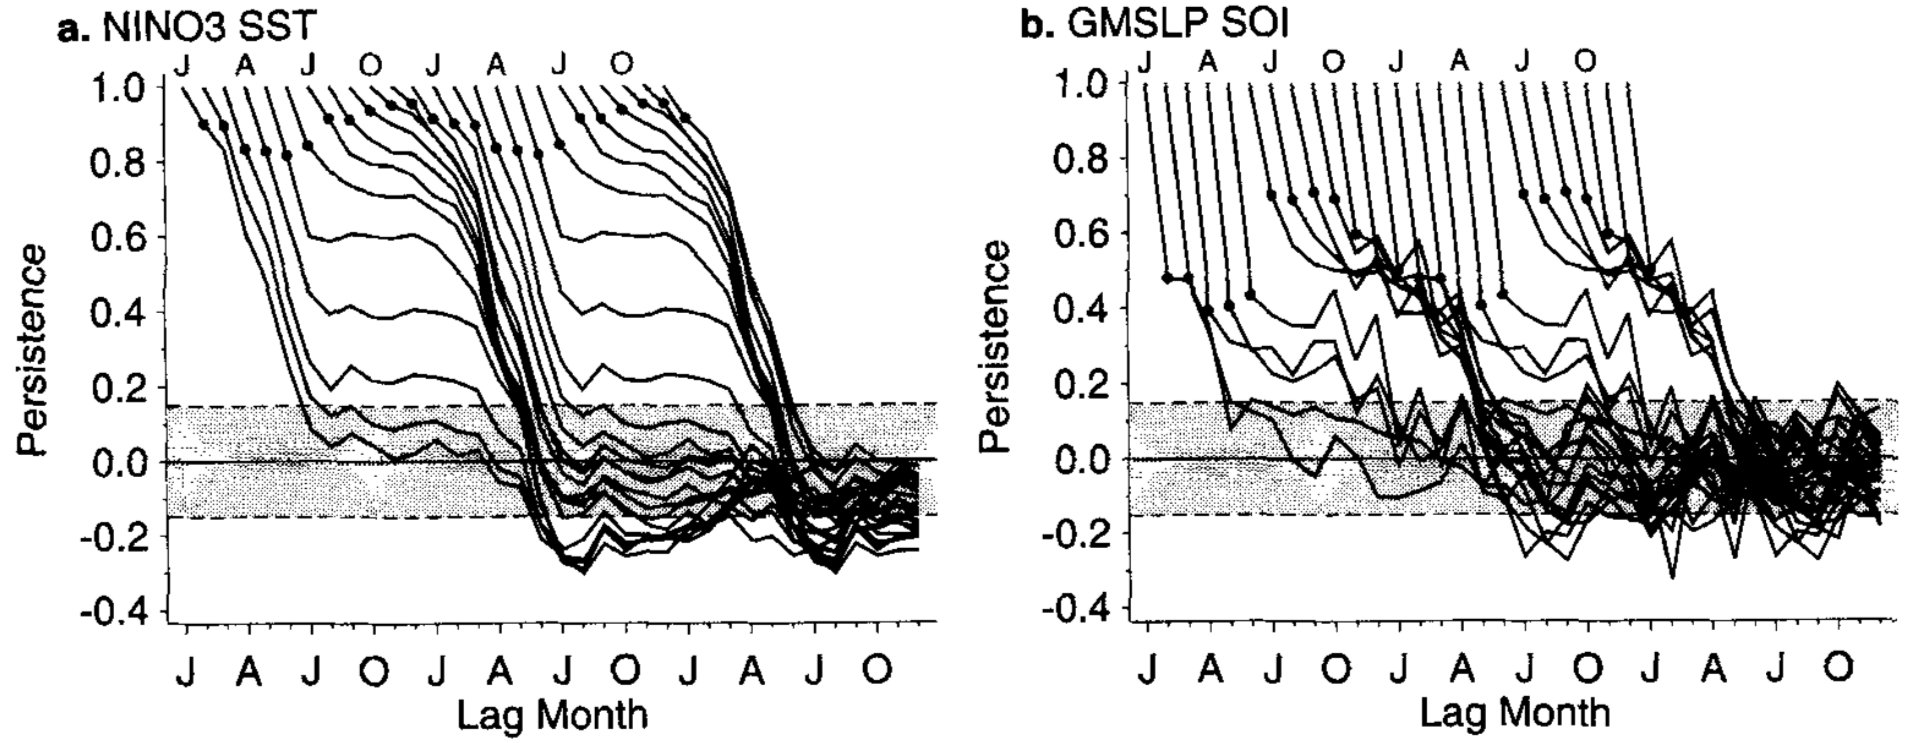
\includegraphics[width=\textwidth]{data/persistence_sst_soi}
\caption[Persistence]{Data showing persistence between different months of the year (from \citealt{torrence1998annual}): (a) Persistence of NINO3 surface sea temperature (SST) with each curve shifted to line up with the starting month on the top axis (JAJO=January, April, July, October), and the corresponding lag month on the lower axis. The black dots show the lag-1 persistence, and all twelve curves for one year were repeated for clarity; (b) Same analysis applied but for the GMSLP Southern Oscillation Index (SOI). The SPB is seen emerging from March and lasting till $\sim$May.}
\label{fig:persistence_sst_soi}
\end{figure}

\noindent
Examinations of the correlation between ENSO data sets through autocorrelation and persistence provides one method for identifying the predictability barrier \citep{torrence1998annual}. The autocorrelation of a time series is the correlation between itself and a duplicate of the data which is time-lagged. Analyses of monthly sea level pressures across the Pacific Ocean yields the SST and Southern Oscillation Index (SOI) to have high autocorrelations which agrees with general observation that ENSO events normally persist for several months \citep{trenberth1976spatial}. Persistence focuses on the fixed-phase correlation between different months within a single time series. Contrasting with autocorrelation which is independent of the starting month, persistence demonstrates potential seasonal changes in the correlations between one month and the next \citep{troup1965southern}. Analysis by \cite{torrence1998annual} of NINO3 SST and GMSLP SOI data indicates that persistence has distinct, regular structure which is phase locked to an annual cycle (Fig. \ref{fig:persistence_sst_soi}). Regardless of starting month, the persistence has a rapid decline in the March--May period which can be attributed as the manifestation of the spring predictability barrier. \\
% words: 169

\begin{figure}
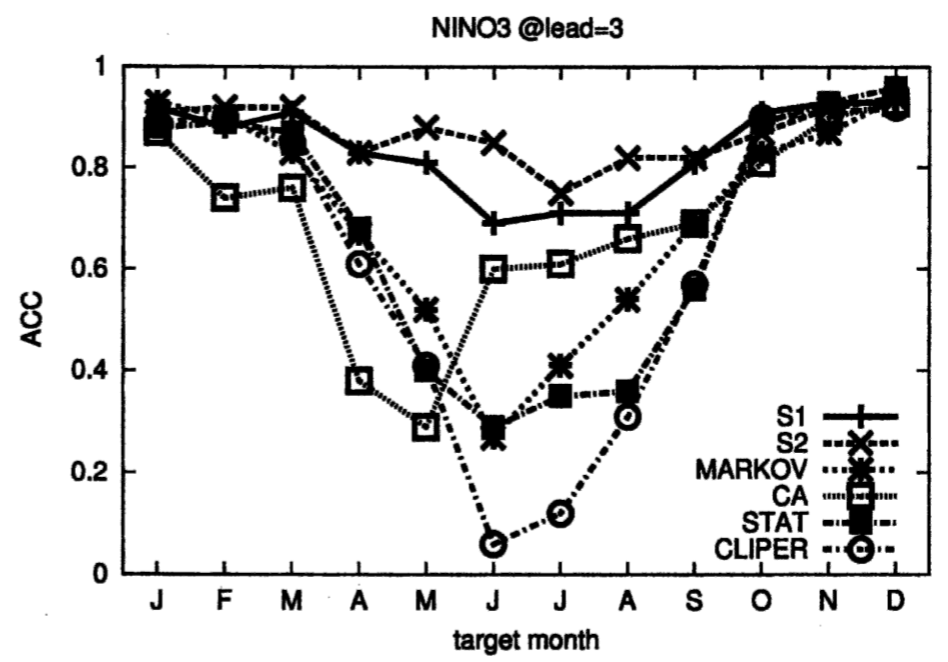
\includegraphics[width=0.6\textwidth]{data/ecmwf_data}
\caption[Persistence]{Plot of the anomaly correlation coefficients of six dynamical and statistical models (S1, S2, MARKOV, CA, STAT, CLIPER) against the months of the year. This demonstrates the skill in predicting monthly Ni\~{n}o-3 index with a lead time of $+3$ months \citep{jan2005did}. The emergence of the SPB appears to occur at different times if non-combined individual models are tested.}
\label{fig:ecmwf_plot}
\end{figure}

With the SPB apparent from observational data, it would be logical to consider where the barrier occurs in theoretical modelling. Performing an investigation with dynamical and statistical models, these frameworks often have origins in seasonal forecasting which make them ideal in ENSO forecasting because they couple the dynamics of the atmosphere, ocean, and land. \cite{jan2005did} tested the skill of six models which were adapted from research by the European Centre for Medium-Range Weather Forecasts (ECMWF). It became apparent that whilst the SPB does arise in the modelling, it appeared to emerge at different times within the year (Fig. \ref{fig:ecmwf_plot}). However it was suggested that this was just an effect of testing the ECMWF models individually, if combinations of the models (multi-model ensembles, MMEs) were used, the results may have better aligned with the data and the variability in barrier period reduced. \\
% words: 141

Similarly, \cite{jin2008current} investigated and analysed the performance in ENSO prediction for other types of coupled general circulation models (CGCMs). They measured that the forecast skill of individual models and MMEs depended strongly on ENSO phase, ENSO intensity, and on the starting season. For forecasts which began in February or May, the skill appeared to drop more sharply than predictions made in August or November. This is yet again a demonstration of the SPB and further highlights the need to understand this limitation within ENSO modelling.
% words: 85

\section{Overcoming the spring predictability barrier}
\subsection{Parameter and initial errors in the Zebiak-Cane model}
\begin{figure}
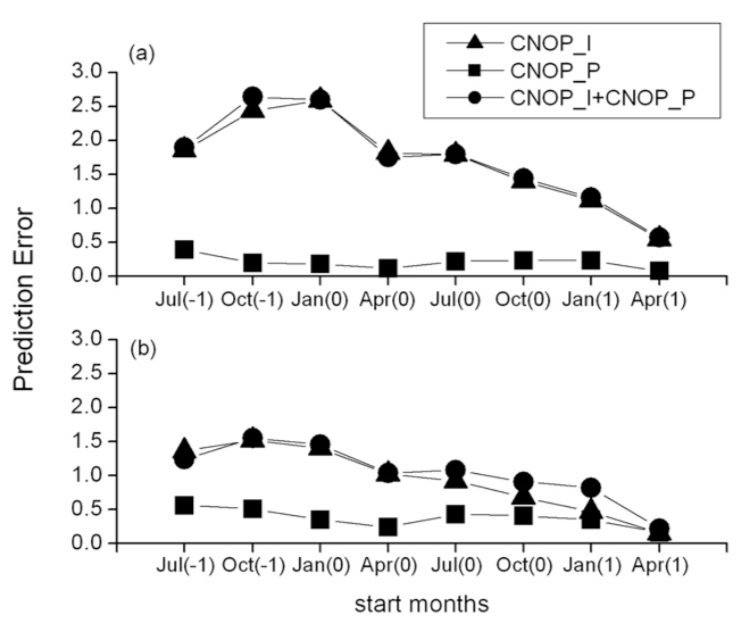
\includegraphics[width=0.6\textwidth]{data/cnop}
\caption[CNOP]{Plots of the mean prediction errors for 16 El Ni\~{n}o events with a lead time of 12 months for each starting month: (a) prediction errors caused by CNOP-I errors, CNOP-P errors, and their combined mode with an initial constraint of $\mid \mid u_0 \mid \mid _\alpha \leq 0.8$; (b) same analysis but with $\mid \mid u_0 \mid \mid _\alpha \leq 0.4$ \citep{yu2012does}. Demonstrating the weakened emergence of the SPB depending on if a parameter-error or initial-error masked system is used.}
\label{fig:cnop}
\end{figure}

\noindent
As described, the SPB is a prevalent characteristic of ENSO forecasts which exists in climate data, and in statistical and coupled models. Whilst it may not be feasible to entirely eliminate the barrier from predictions, it would be beneficial to reduce its effect. A potential line of inquiry is understanding the initial and parameter errors within the ZC model which leads to the SPB. Through adopting an approach of conditional nonlinear optimal perturbations (CNOP), the errors can be isolated and their impact on the SPB quantified \citep{duan2009exploring}. This method identifies the optimal error perturbations (initial or parameter) in the ZC model within given constraints through reducing evolution equations \citep{mu2010extension}. Applications of CNOP in retrospective forecasts reveals that prediction errors for a parameter-error only system (CNOP-P) are small which generates a weakened SPB, on the other hand an initial-error only framework (CNOP-I) produces significant SPBs (Fig. \ref{fig:cnop}). If both are coupled together as found in a realistic system, then the prediction errors are weighted by the CNOP-I results and a substantive SPB arises. \\
% words: 172

To reduce the effect of CNOP-I uncertainties on the prediction results, it is suggested that an ensemble forecast technique based on a multi-initial condition ensemble could be used in predicability studies and operational forecasts \citep{kirtman2001current}. However this would require an alternative prediction model and there is yet to be one which accurately considers enough climate system components. 
% words: 57

\subsection{Stochastic forcing and westerly wind bursts}
\noindent
Utilising the prediction model, considerations of the established initial-error values allows for the strength of the SPB to be reduced. Nonetheless the origins and fundamental mechanisms of the barrier are still in debate and there is yet to be a single conclusive argument. There are two main hypotheses which attempt to justify the low ENSO prediction skill during spring: the first is the original ZC model which suggested that the air-sea coupling strength is the weakest during the boreal spring \citep{Zebiak:1987aa}, the second compares the seasonality of the SST anomaly (SSTA) variance to that of the stochastic noise forcing which provides an indicator of the SPB \citep{webster1992monsoon, xue1994prediction}. On the other hand, there is potential for alternatives theories which utilise different climate phenomena such as Westerly Wind Bursts (WWBs) to solve ENSO forecast skill seasonality. \\
% words: 135

\begin{figure}
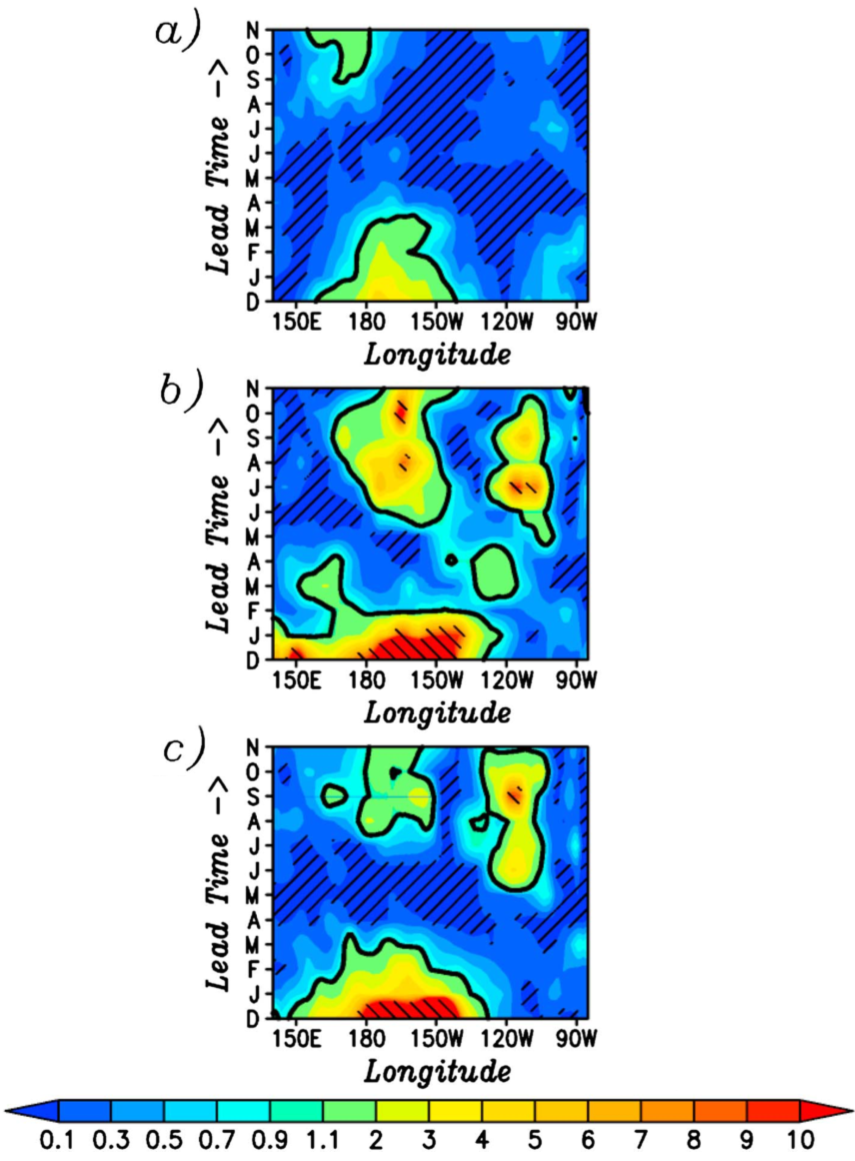
\includegraphics[width=0.7\textwidth]{data/wwbs}
\caption[WWBs]{Composites of the signal-to-noise ratio for zonal wind stress across the equatorial Pacific for (a) observed, (b) idealised CCSM3 model without WWBs, and (c) idealised CCSM3+WB which includes WWBs \citep{lopez2014wwbs}. The inclusion of WWBs in climate models could improve the predictability of ENSO events.}
\label{fig:wwbs}
\end{figure}

The inclusion of parameterised WWBs in prediction experiments is motivated because of their occurrence in nature and the need to model a more realistic system rather than an idealised one. Incorporating wind bursts into the Community Climate System Model Version 3 (CCSM3+WB; \citealt{collins2006community}) allows for the observed SSTA to be retrospectively predicted. Producing yearly forecasts for 1982--1998 provides a large sample for prediction experiments and model testing \citep{lopez2014wwbs}. These forecasts show that there is a significant decrease in the signal-to-noise (S/N) ratio during the spring period for zonal wind stress across the equatorial Pacific. This S/N decrease is most notable in observational data (Fig. \ref{fig:wwbs}(a)) and in CCSM3+WB models (Fig. \ref{fig:wwbs}(c)), however it is also prevalent in non-WWB models (Fig. \ref{fig:wwbs}(b)) but with less strength. Analysing correlation statistics for real prediction experiments shows that there is a pronounced drop in skill with the WWB model during spring, whereas the change is more dramatic when there are no WWBs. These results imply that the SPB is influenced by the existence of WWBs and to produce better skilled predictions, climate models should account for them.
% words: 183

\section{Conclusions}
\noindent
To summarise, understanding the mechanisms for ENSO prediction and formation is currently limited as models such as ZC simplify the coupling between the atmosphere and ocean which limits their applicability to non-regular El Ni\~{n}o events. An additional challenge arises in the form of the SPB where the predictive skill across March--May is low when compared to predictions originating from other times in the year. This barrier is evident from data and modelling, but there is yet to be a conclusive model which explains why it exists. Current research suggests that the barrier may be related to weak climate coupling during spring or it may arise due to stochastic noise forcing. However, these models fail to account for WWBs to be the potential source of the seasonality in ENSO forecast skill. Incorporating them into prediction models suggests the SPB may be materialising due to the presence of the WWBs and that they are an important component in ENSO dynamics. \\
% words: 158

\textit{Final word count: 1947}

% Identify the topic 
% Identify issues with the model
% Identify data and evidence that suggests model needs revising
% Suggest and defend new model or models

\clearpage

%\nocite{wang2017nino}
%\nocite{ruddiman_climate}
\bibliographystyle{agsm}
\bibliography{el_nino}

\end{document}